Consider an economy with $N$ agents, evolving in the time interval $[0,T]$.
Each agent is described at time $t$ by his wealth $A_t$ and his skill level $H_t$,
with $(A_t, H_t) \in \Omega = \mathbb{R} \times \mathbb{R}^+$ for every $t \in [0,T]$.
Agents control their consumption $c_t \in \mathbb{R}^+$, and the proportion of time dedicated to working $u_t \in [0,1]$. 
We assume that the proportion $1 - u_t$ of time not used to working is used to improve their skill level. 
Moreover, for every $i \in \{1,...,N\}$,  agent $i$ faces the following optimization problem:
\begin{equation}\label{education_model:representative_agent_optimization}
\begin{cases}
        \sup\limits_{(u,c) \in \mathcal{U} \times \mathcal{C}}\mathbb{E} [ \int_0^T f_c(c^i_s) + f_u(u^i_s) ds + Q(A^i_T) ], \text{ s.t.}\\
        d A^i_t = \left[ (\bar r_t - \delta) A^i_t + \bar w_t H^i_t u^i_t - c^i_t  \right] dt + \sigma_a A^i_t d W^{a,i}_t,\\
        d H^i_t = (H^i_t)^\xi g(1 - u^i_t) dt + \sigma_h H^i_t d W^{h,i}_t.
\end{cases}
\end{equation}
The term $f_c(c_s)$ is a running utility for consumption, whereas $f_u(u_s)$ is a running utility for proportion of time spent working.
The term $Q(A_T)$ represents utility over terminal wealth.

The agent's wealth $A_t$ evolves with a drift term $\left[ (\bar r_t - \delta) A_t + \bar w_t H_t u_t - c_t  \right] dt $ and a noise term $\sigma_a A_t d W^a_t$.
The drift term is composed of interest returns over current wealth given by $(\bar r_t - \delta) A_t$, wages $\bar w_t H_t u_t$  proportional to time dedicated to working and a reduction on wealth due to consumption given by $c_t$. The interest rate of the economy $\bar r_t$ and the wage rate per time per skill $\bar w_t$  are determined endogenously through mean field interactions, whereas $\delta$ is a given depreciation rate. 

The agent's skill level $H_t$ evolves through time with a drift term $H^\xi_t g(1 - u_t) dt$ and a noise term $\sigma_h H_t dW^h_t$.
The function $g$ represents the effectiveness of time $1 - u_t$ employed in improving skill level,
 whereas the term $H_t^\xi$ captures the impact of current skill level in effectiveness of effort.
 For $\xi > 0$, higher skill levels lead to higher effectiveness.
  However, for $\xi < 0$, higher skill levels lead to lower effectiveness.
  As for $\xi = 0$, the effectiveness is indifferent to skill level.

The noise terms $\sigma_h H_t dW^h_t$ and $\sigma_a A_t dW^a_t$ are driven by independent brownian motions ${(W^h_t)}_{t \in [0,T]}$ and ${(W^a_t)}_{t \in [0,T]}$.
We consider that each agent has independent noise.

Interaction between agents is mediated through $\bar r_t$ and $\bar w_t$.
These values depend on aggreates of the agent's states and on the production function of the economy as folows:
Suppose that the economy has a Cobb-Douglas production~\cite{cobb1928theory} function $F$ which depends on average wealth $\bar a_t$ 
and on the effective supply of skilled labor $\heff_t$.
At time $t$, the agents are distributed over $\Omega$ with a measure $\mu^N_t \in \mathcal{P}(\Omega)$ given by
\[
\mu^N_t = \frac{1}{N} \sum_{i = 1}^N \delta_{(A^i_t, H^i_t)}.
\]
Average wealth is then given by
\[
\bar a(\mu^N_t) \coloneqq \int_\Omega \, a \, d\mu^N_t (a,h),
\]
whereas the effective supply of skilled labor is given by
\[
\heff(\mu^N_t) \coloneqq \int_\Omega \, u(a,h) h \, d\mu^N_t (a,h).
\]
The interpretation for average wealth is straightforward.
The effective supply of skilled labor is a weighted average of skill over the population, where the weights $u(a,h)$ are the proportion of time dedicated to work as a function of the state $(a,h)$.
It is clear that $\heff(\mu^N_t) \leq \int_\Omega  h \, d\mu^N_t (a,h) \coloneqq \bar h(\mu^N_t)$, where equality holds if every agent dedicates his whole time to work.

At economic equilibrium, the interest rate and the wage rate are equal to their marginal increase in production~\cite{cobb1928theory}, that is
\[
\bar r(\mu^N_t)= \partial_a F(\bar a(\mu^N_t), \heff(\mu^N_t)), \quad \bar w(\mu^N_t)= \partial_h F(\bar a(\mu^N_t), \heff(\mu^N_t)).
\]
To simplify the notation, we denote
\[
\bar a_t \coloneqq \bar a(\mu^N_t), \heff_t = \heff(\mu^N_t), \bar r_t = \bar r(\mu^N_t), \bar w_t = \bar w(\mu^N_t).
\]
For a production function $F(a,h) = C a^\beta h^{1 - \beta}$, $0 \leq \beta \leq 1$, we have
\[
\bar r_t = C \beta {\bar a_t}^{\beta - 1} {(\heff_t)}^{1 - \beta} = \beta \frac{F(\bar a_t, \heff_t)}{\bar a_t},
\]
and
\[
\bar w_t = C (1 - \beta) {\bar a}_t^{\beta} {({\heff}_t)}^{ - \beta} = (1 - \beta) \frac{F (\bar a_t, \heff_t)}{\heff_t}.
\]
An agent at state $(a,h)$ will receive $\bar r_t a$ as interest and $\bar w_t u(a,h) h$ as wages.
Integrating over the population's density measure $\mu^N_t$ leads to
\[
    \int_\Omega \bar r_t a \, d\mu^N_t(a,h) = \beta F(\bar a_t, \heff_t),\quad \int_\Omega \bar w_t u(a,h) h \, d\mu^N_t(a,h) = (1 - \beta) F(\bar a_t, \heff_t).    
\]
This means that the economy is closed in the sense that everything that is produced is distributed either as interest or as wages.

For a given population evolution described by a measure flow $\mu_t \in C([0,T],\mathcal{P}(\Omega))$, the optimal control problem~\eqref{education_model:representative_agent_optimization} is a standard stochastic optimal control problem.
However, the optimal trajectories for this optimization problem define a measure flow, which we denote $O(\mu_t)$   
A Nash equilibrium for the mean-field limit of the game is a measure flow $\mu^*_t$ such that $ \mu^*_t = O(\mu^*_t)$, that is, the flow is induced by the optimal trajectories of its own associated optimization problem.

Coupling the HJB equation describing the value function for the optimization problem and the FKP equation describing the measure flow, we arrive at System~\eqref{education_model:mfg_analytic_system}, which describes Nash equilibria for the limit of the game as $N \to \infty$~\cite{cardaliaguet2010notes}.
The function $V: [0,T] \times \Omega \mapsto \mathbb{R}$ is the value function for the game at the Nash equilibrium,
whereas the probability measure flow $\mu: [0,T] \times \Omega \mapsto \mathbb{R}$ describe the time evolution of the  population density over the state space $\Omega$.
\begin{equation}\label{education_model:mfg_analytic_system}
    \begin{cases}
        \partial_t V + (\bar r  - \delta) a \partial_a V + \HH_u(h, \partial_a V, \partial_h V)  + \HH_c(\partial_a V) + \frac{1}{2} \sigma_a^2 a^2 \partial_{aa} V + \frac{1}{2} \sigma^2_h h^2 \partial_{hh} V = 0,\\
        \partial_t \mu + \partial_a \left( \left[ (\bar r - \delta) a + \partial_p \HH_u(h, \partial_a V, \partial_h V) + \partial_p \HH_c(\partial_a V) \right] \mu \right) 
        \\ \quad \quad \quad \quad \quad \quad \quad \quad \quad + \partial_h \left( \partial_q \HH_u(h, \partial_a V, \partial_h V)\, \mu\right)  - \frac{1}{2} \sigma_a^2 \partial_{aa} (a^2\mu) - \frac{1}{2} \sigma^2_h \partial_{hh} (h^2\mu) = 0,\\
        \mu(0,a,h) = \mu_0,\quad V(T,a,h) = Q(a)
    \end{cases}
\end{equation}
where
\begin{equation}
    \begin{cases}
        \HH_u(h,p,q) = \sup\limits_{u} \left \{ h^\xi \, g(1 - u)\, q + h u \, \bar w (\mu)\, p + f_u(u)\right\},\\
        \HH_c(p) = \sup\limits_{c} \left \{  f_c(c) - c \, p \right \}
    \end{cases}
\end{equation}

The Nash equilibria can also be formulated as the solution to a system of 
McKean-Vlasov Forward Backward Stochastic Differential Equations (MV-FBSDE),
by applying the Stochastic Maximum Principle to the optimization problem~\eqref{education_model:representative_agent_optimization}~\cite{carmona2018probabilistic}.
Suppose there exist functions $\hat u : \mathbb{R}^+ \times \mathbb{R} \times \mathbb{R} \mapsto [0,1] $ and $\hat c : \mathbb{R} \mapsto \mathbb{R}^+$ such that
\begin{equation}
    \begin{cases}
         \left \{ h^\xi \, g(1 - {\hat u}(h,p,q))\, q + h {\hat u}(h,p,q) \, \bar w (\mu)\, p + f_u({\hat u}(h,p,q))\right\} = \HH_u(h,p,q),\\
         \left \{  f_c({\hat c}(p)) - {\hat c}(p) \, p \right \} = \HH_c(p)
    \end{cases}
\end{equation}
Let $\hat u_t \coloneqq \hat u(H_t,P_t,Q_t)$ and $\hat c_t \coloneqq \hat c(P_t)$.
Then solutions $(A_t, H_t, P_t, Z^p_t, Q_t, Z^q_t)$ for the MV-FBSDE
\begin{equation}\label{education_model:mfg_fbsde_system}
    \begin{cases}
        d A_t = \left[ (\bar r_t - \delta) A_t + \bar w_t H_t {\hat u}_t - {\hat c}_t  \right] dt + \sigma_a A_t d W^a_t,\\
        d H_t = H^\xi_t g(1 - {\hat u}_t) dt + \sigma_h H_t d W^h_t,\\
        d P_t = -\left[ (\bar r_t - \delta) P_t + \sigma_a Z^p_t \right]dt + Z^p_t d W^a_t,\\
        d Q_t = - \left[ \xi H_t^{\xi - 1} g(1 - {\hat u}_t ) Q_t + {\bar w} {\hat u}_t P_t + \sigma_h Z^q_t \right] dt + Z^q_t d W^h_t,\\
        \mathcal{L}(A_0, H_0) = \mu_0, \, P_T = \partial_a Q(A_T), Q_T = 0,
    \end{cases}
\end{equation}
describe Nash equilibria for the mean field limit of the game.
Note that the dependency of the dynamics on the law $\mathcal{L}(A_t,H_t)$ is implicit in $\bar r_t$ and $\bar w_t$.
Solutions for~\eqref{education_model:mfg_analytic_system} and~\eqref{education_model:mfg_analytic_system} are related through $\mathcal{L}(A_t, H_t) = \mu_t$, $P_t = \partial_a V(t,A_t,H_t)$ and $Q_t = \partial_h V(t,A_t,H_t)$.

\subsection{Numerical Illustration}
        A deterministic, simplified version of the model was simulated through Picard iterations.
        
        \textcolor{red}{describe in more details what you did.}
        
        We aim to use this simulation as a benchmark for further studies.        
        Let's set \textcolor{red}{Parameter table}
        %$$g(1- u) = (1 - u),\,\xi = 0,\, \delta = 0.05, \, k = 0.5,\, f_c(c) = \log(c), f_u(u) = -\frac{\alpha}{2} u^2, Q(a) = a.$$        
        In this case, we have 
        \begin{equation}
            \begin{cases}    
            \HH_u(h,p,q) = \sup\limits_{u} \left\{ (1 - u)q + \bar w_t h u p - \frac{\alpha}{2} u^2 \right\},\\
            \HH_c (p) = \sup\limits_{c} \left\{ \log(c) - cp \right\}.
            \end{cases}
        \end{equation} 
        Two scenarios are simulated: $\alpha = 0.5$ and  $\alpha = 2$ representing a lower and a higher preference to education versus work, respectively.

        \textcolor{red}{Try to solve PDEs using DGM}
        \textcolor{red}{Change format of plots to suit document.}
        %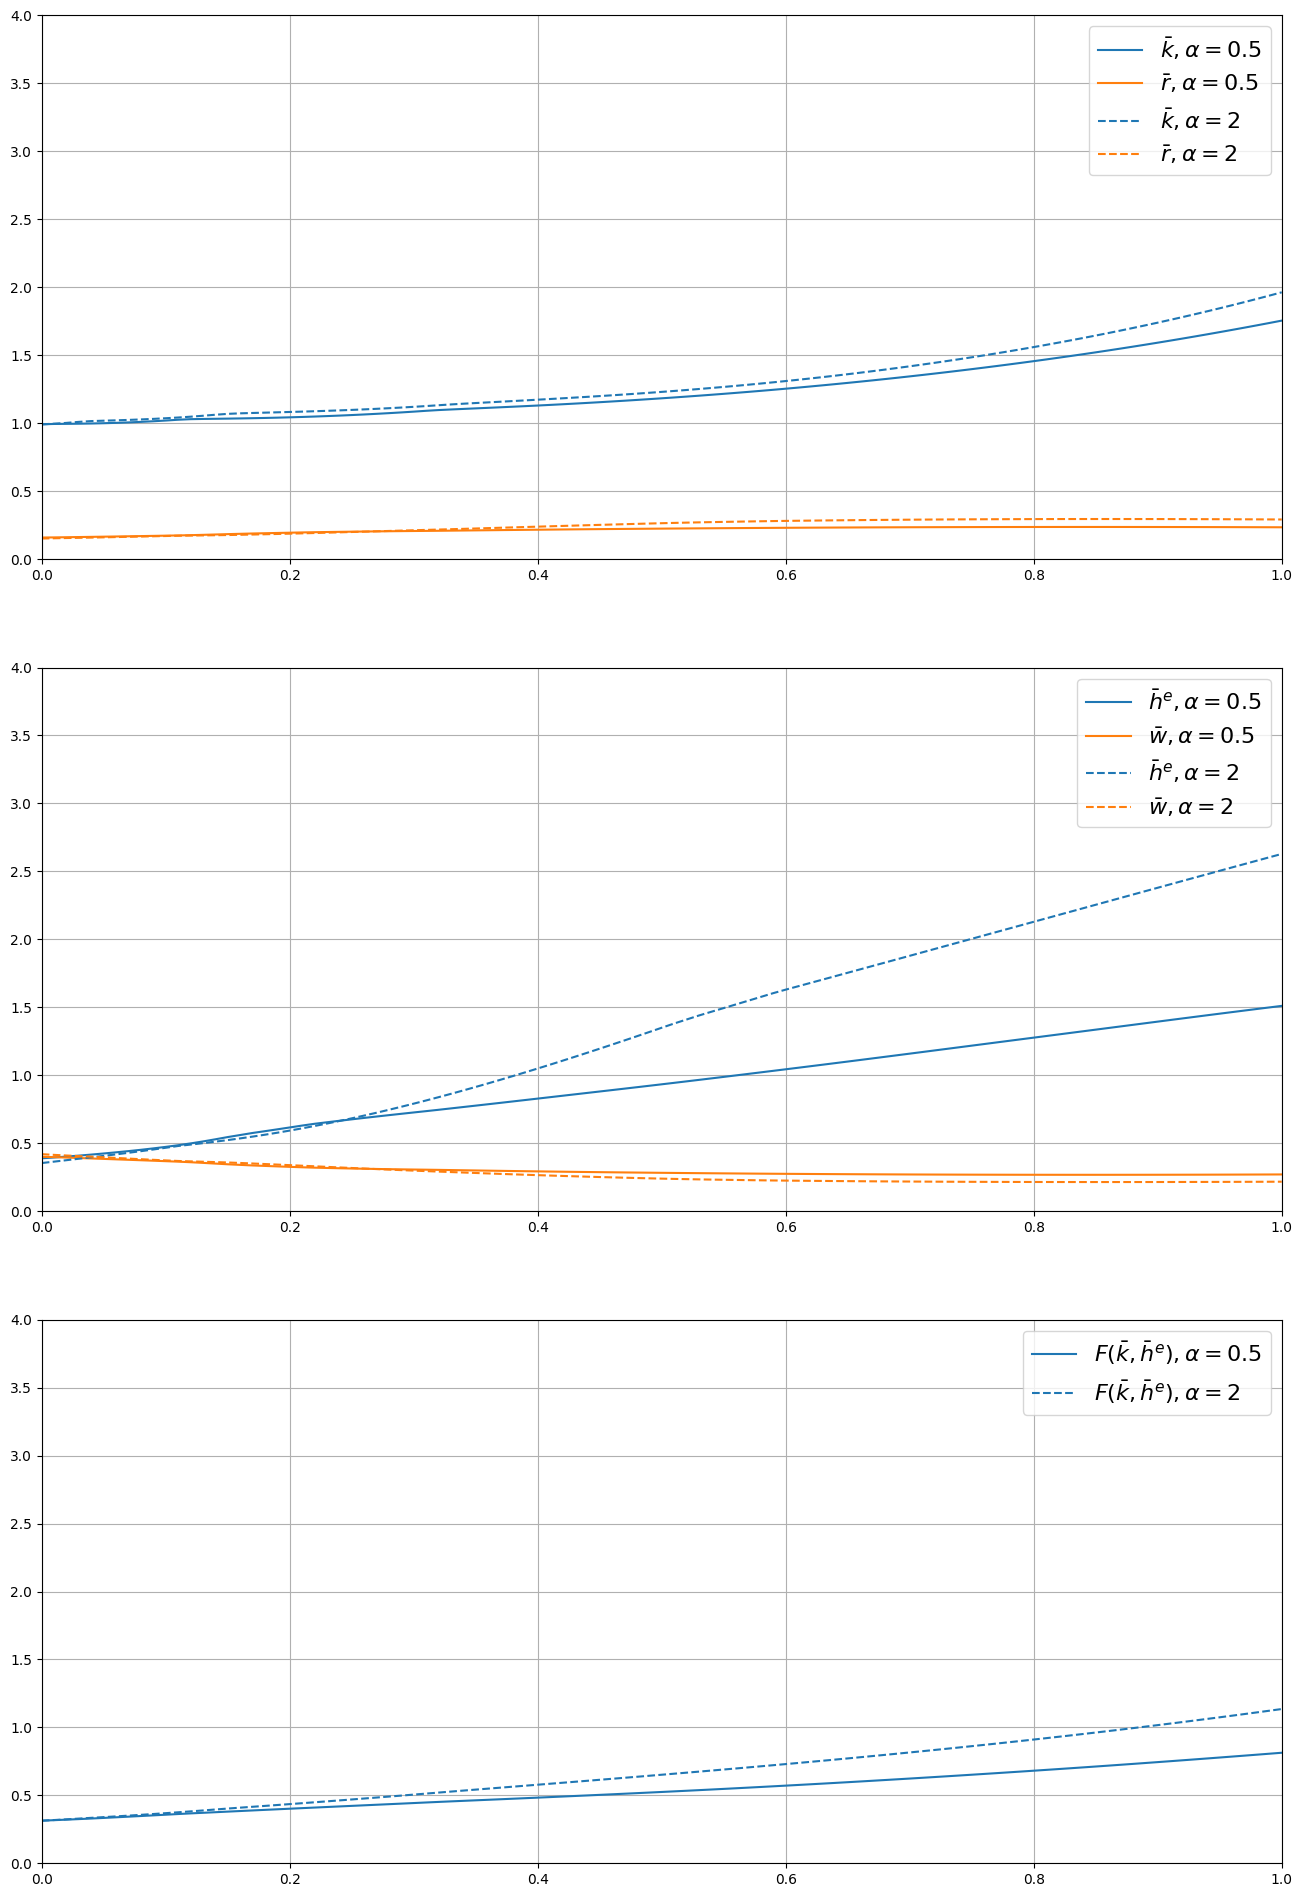
\includegraphics[width=\textwidth]{simulations_mfg.png}